\documentclass{article}
\usepackage[utf8]{inputenc}
\usepackage{graphicx}
\usepackage[margin=1in]{geometry}
\usepackage{hyperref}

\author{Bijan Varjavand}
\title{Solo Lab Write-up}

\begin{document}

\maketitle
\ \\[2in]

\section{Abstract}
\centering
WOWOWOOWOWOWOW

\clearpage

what people use xrd for, how xrd works (bragg's law, penetration)
\raggedright
\section{Introduction}

This lab blahblah.

\subsection{The Unit Cell}

The unit cell has multiple different conformations. Examples include body-centered cubic(BCC) and face-centered cubic(FCC).

\begin{figure}[h]
	\begin{minipage}{0.5\textwidth}
		\centering
		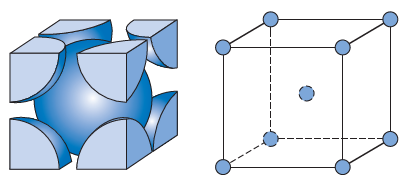
\includegraphics[scale=.5]{bcc.png}
	\end{minipage}
	\begin{minipage}{0.5\textwidth}
		\centering
		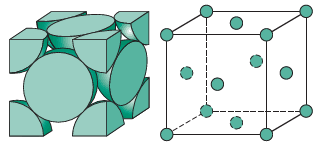
\includegraphics[scale=.6]{fcc.png}
	\end{minipage}
	\caption{Left: BCC, Right: FCC}
\end{figure}

One important aspect of a unit cell is its burgers vector and dense plane. These values indicate the direction of most dense packing. Notation for these dense direction is in miller indices (h, k, l, where hkl are orthogonal directional axes). Not only that, but due to symmetry of unit cells, the burgers vector is a family of h, k, and l values. For example, the family $\{1\ \overline{1}\ 0\}$ includes all hkl values that, when squares are added, equal 1. This is actually the burgers vector for FCC unit cells, and a one is shown below.

\begin{figure}[h]
	\centering
	\includegraphics[scale=.6]{"dense direction".png}
	\caption{Dense plane for FCC unit cell - \{1 $\overline{1}$ 0\}}
\end{figure}

One can see that, in the unit cell space, the "dense direction" is easily found as the highest density of atoms in a specific direction. This is also the direction that slips form across most easily due to the close stacking of atoms. This is due to stacking fault energy in that direction being the lowest, as the maximum displacement between atoms is lowest(due to distance between atoms being the lowest as well).

\ 

Dislocations are linear imperfections in a crystal structure, and occur along the Burgers vector. The more dislocations are present in a material, the more difficult it is for the material to be bent and shaped. This is due to the dislocations.

\subsection{Grain Boundaries} 

The orientation of h, k, and l vectors are linked to each other within each grain. At the grain boundary, dislocation lines separate the slight change in orientation of h, k, and l vectors. These lines are visible to optical microscopy and can be counted - exactly the contents of this section of the lab. A fundamental diagram of grain boundaries is seen below

\begin{figure}[h]
	\centering
	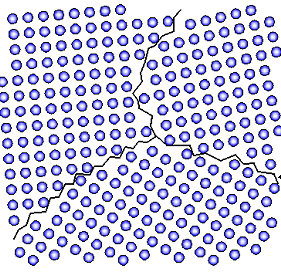
\includegraphics[scale=.6]{grain.png}
	\caption{black lines are the dislocations separating grains. \url{<http://www.engineeringarchives.com/img/les\_ matsci_surfacedefects_1.png>}}
\end{figure}
\ \\[1.35in]

We can see how the orientation of the crystal structure has shifted in between grains. Taking a more applied look at this concept, we can see the grain structure of three of our samples of steel. Taking a look at the visual structures of the 3 samples,

\begin{figure}[h]
	\begin{minipage}{0.32\textwidth}
		\centering
		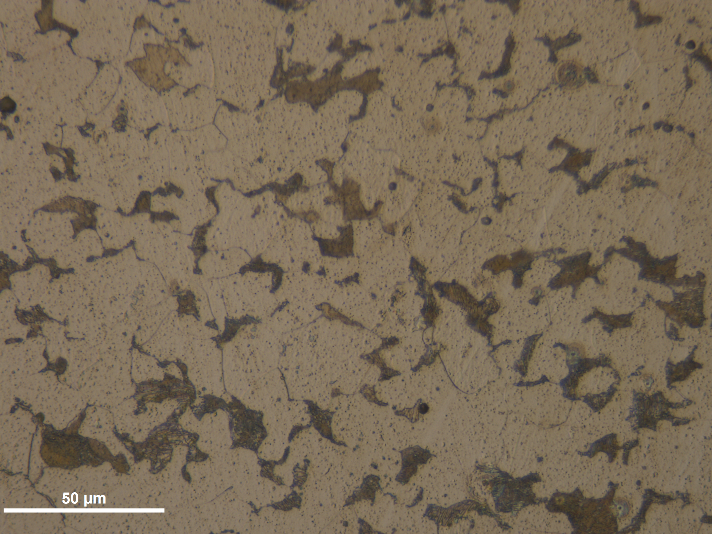
\includegraphics[scale=.5]{TransAnnealedSteel.png}
	\end{minipage}
	\begin{minipage}{0.32\textwidth}
		\centering
		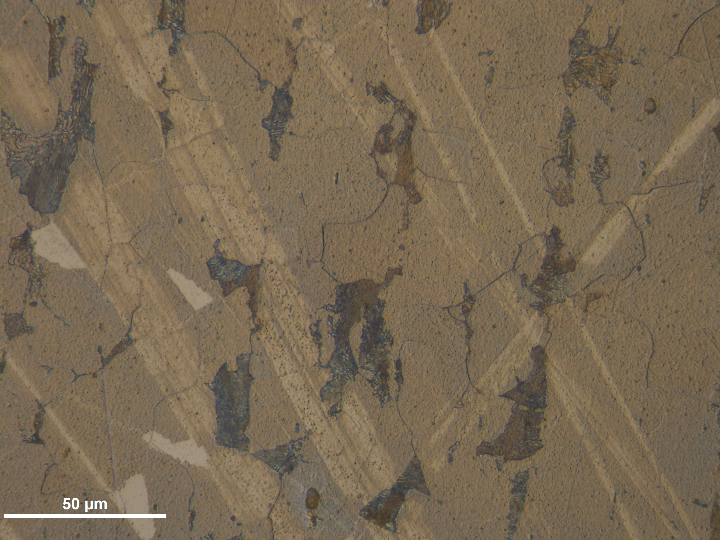
\includegraphics[scale=.5]{LongAnnealedSteel.png}
	\end{minipage}
	\begin{minipage}{0.32\textwidth}
		\centering
		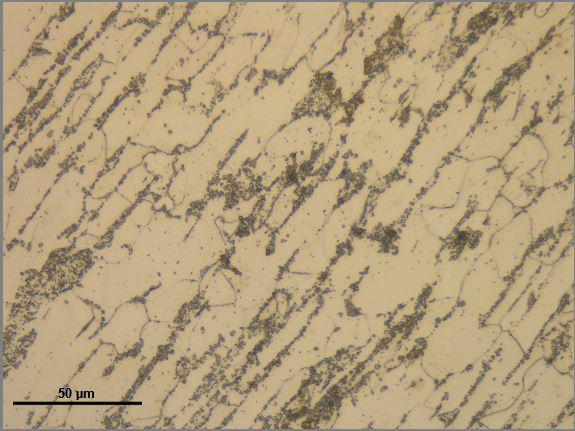
\includegraphics[scale=.28]{LongARSteel.png}
	\end{minipage}
	\caption{Left: Transverse Annealed, Mid: Longitudinal Annealed, Right: Longitudinal As Received}
\end{figure}

we can see differences in the grain structure, specifically in their shape and orientation. The longitudinal cross-section obviously will have longer grains, while the transverse cross-section will have more evenly shaped grains. An important distinction between these materials, other than the direction of the grains, is whether or not they have been annealed. The process of annealing is very well-understood in the field of materials engineering - allowing a material to cool slowly after it is heated will make it softer and more easily cut. This is because once the material is heated above its re-crystallization temperature and allowed to cool, the material recrystallizes and has a reduced number of dislocations.

\subsection{Our Samples}

Specifically, the samples that were used include as received steel 1018, annealed steel 1018, and titanium 6-4. We also observed the x-ray diffraction pattern of aluminum 6061. Discussion of the importance of each sample is important for understanding the scope of the lab.

The 1018 in 1018 steel is from the composition of the material. It is made of 0.18\% Carbon, 0.6-0.9\% Manganese, and 98.82-99.22\% Iron. Due to its low carbon content, it has good weldability and a good balance of toughness, strength, and ductility. It is used in a huge variety of applications, including most casting processes.

Titanium 6-4 has a more complicated composition, but the notable elements are Aluminum(6\%) and Vanadium(4\%). The main use for these materials is in cogs among other applications due to their high toughness and tensile strength even at high temperatures. They also have a low weight. Additionally, there are uses for this material in the biomedical field due to its low weight and compatibility with bone and tissue.

Aluminum 6061 is composed of Aluminum, Magnesium, Silicon, Manganese, and Chromium, while the 6061 is from the 0.60\% weight percent in the specific alloy. One use for this material is in bicycle frames due its extremely low weight. One notable feature of aluminum and its alloys are difficult to anneal, since they will melt almost immediately. One technique to assist in annealing is to leave soap on the material as it will turn black under heat almost immediately, indicating success of the annealing process.

\section{Optical Microscopy}

\subsection{Intro and prep}

Optical microscopy is a technique that uses light to view the sample at high magnification. The main method of generating images at such high magnifications are the use of multiple magnifying lenses as well as a light source. A diagram of the layout can be seen below along with a visual picture:

\begin{figure}[h]
	\begin{minipage}{.5\textwidth}
		\centering
		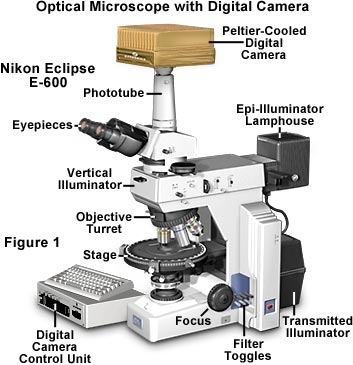
\includegraphics[scale=.3]{optical1.jpg}
	\end{minipage}		
	\begin{minipage}{.5\textwidth}
		\centering
		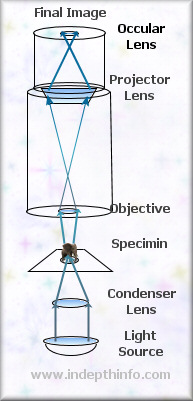
\includegraphics[scale=1.5]{optical2.jpg}
	\end{minipage}
	\caption{Left: A diagram of an optical microscope, Right: A diagram of the travel of light in an optical microscope}
\end{figure}

Preparing my samples to be viewed by the optical microscope was not trivial. The first step after acquiring my sample was to polish it. The complexity with polishing is that one can't use a grit that is too low or high. Grit too low will destroy the features of the sample, while grit too high polishes too inefficiently. Personally, I began with hand-polishing my sample on sand paper, smoothing edges and removing oxidation layers from the needed face. After that, I generated a puck of epoxy with the sample embedded inside. This puck was designed specifically to be fit into the polishing machine. This puck was then polished on the machine, and, using the software's predesigned polishing stages, was polished to an acceptable degree for viewing on the optical microscope.

\subsection{Procedure}

The specific microscope we used utilized the $\textbf{\_\_\_\_\_\_\_}$ software. The first step was to focus the microscope on a lower magnification setting and locate relevant features at acceptable quality (specifically avoiding scratching among other defects). blah. I generated these images, only showing the ones for annealed steel below. The data for the other materials can be easily found in the same directory as this pdf.

\subsection{Results and Observations}

\begin{figure}[h]
	\begin{minipage}{0.32\textwidth}
		\centering
		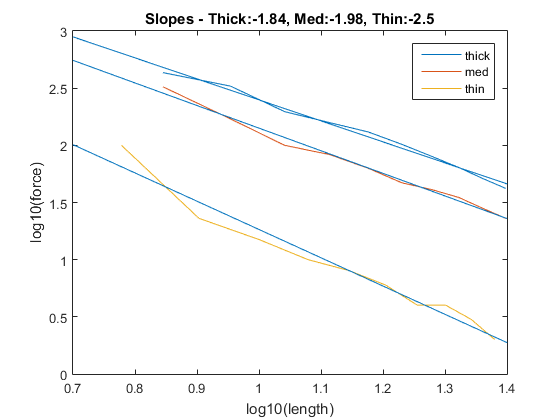
\includegraphics[scale=.3]{Lab1f1.png}
	\end{minipage}
	\begin{minipage}{0.32\textwidth}
		\centering
		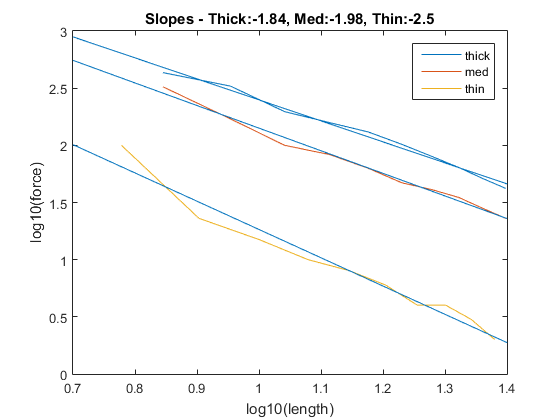
\includegraphics[scale=.3]{Lab1f1.png}
	\end{minipage}
	\begin{minipage}{0.32\textwidth}
		\centering
		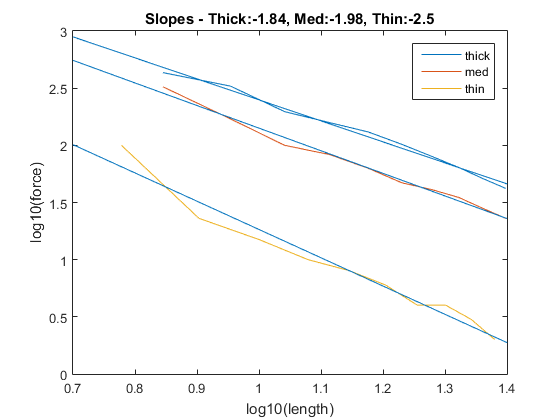
\includegraphics[scale=.3]{Lab1f1.png}
	\end{minipage}
	\caption{Left: SC, Mid: BCC, Right: FCC}
\end{figure}

The first step was to use the grain wizard to automatically calculate the grain index. blah. manual counting. ANSI standard.
$$equation$$
$$value = number$$

Description of relationship between calculated and found values.

\section{X-Ray Diffraction}

\subsection{Intro}

X-Ray diffraction is a great thing that helps us.

\subsection{Procedure}

I did things.

\subsection{Results and Observations}

\begin{figure}[h]
	\begin{minipage}{.5\textwidth}
		\centering
		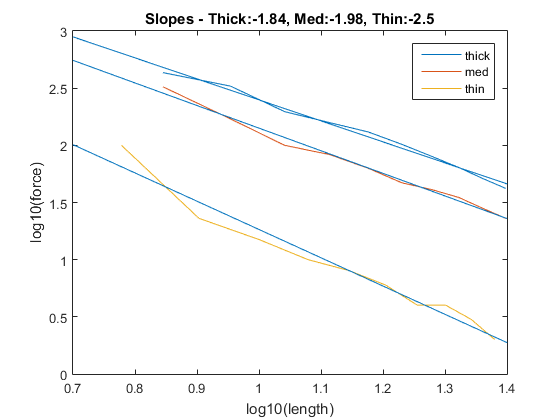
\includegraphics[scale=.3]{Lab1f1.png}
	\end{minipage}		
	\begin{minipage}{.5\textwidth}
		\centering
		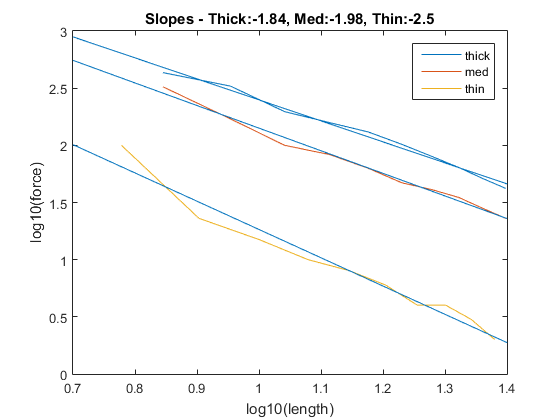
\includegraphics[scale=.3]{Lab1f1.png}
	\end{minipage}
\end{figure}

Wow that's amazing. Look it matches with what I thought.

\end{document}